% ============================================================
%  CHAPTER 3 – System Design
% ============================================================
\chapter{System Design}
\label{ch:system-design}
This chapter divides the work amongst 5 engineering students according to their role presented by their degree. Each of the roles are responsible for a functional section of the design. Section~\ref{sec:functional-flow} covers the functional flow diagrams of the system. Section~\ref{sec:system-architecture} gives the overview of the system design with the top-most architecture, which is then split amongst the five roles in Section~\ref{sec:functional-units} (subsections~\ref{subsec:eeri1-fu1p1} to \ref{subsec:reii-fu1p5}).

\section{Functional Flow Diagrams}
\label{sec:functional-flow}

The flow system operation runs from development, deployment, mounting, operation and maintenance until its decomission or failure as indicated in figure~\ref{fig:ffd-lifecycle}.

\begin{figure}[H]
    \centering
    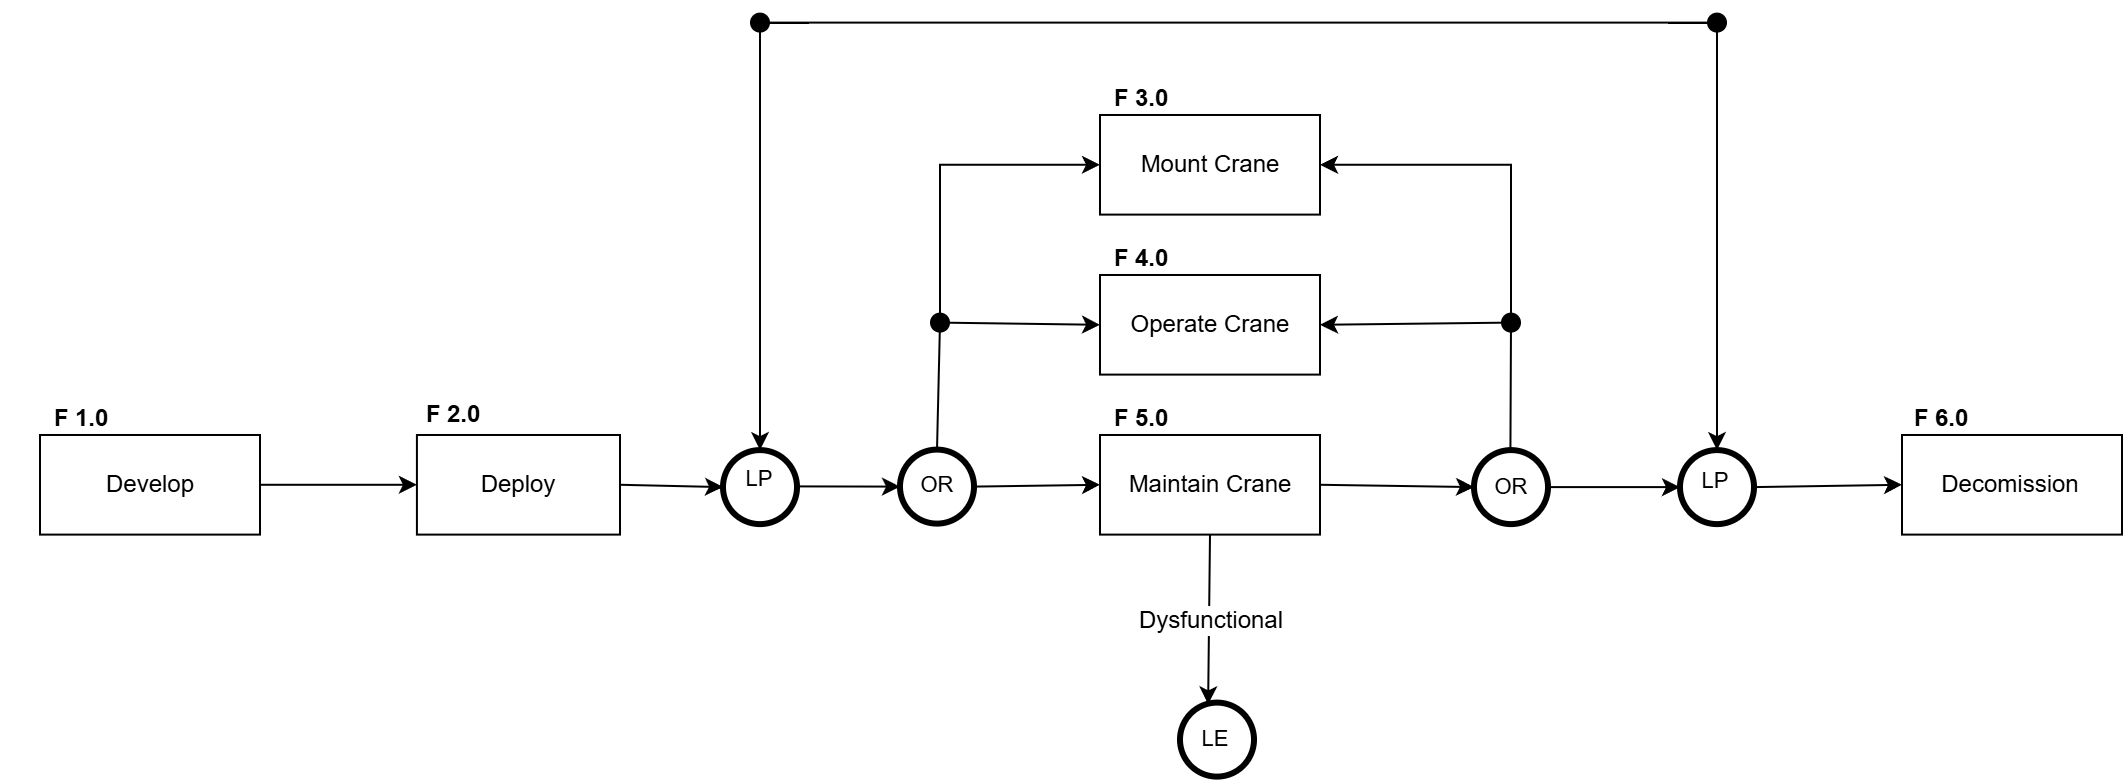
\includegraphics[width = \textwidth]{figures/Fig_LifeCycleofGantryCrane.png}
    \caption{Functional flow diagram illustrating the system life-cycle.}
    \label{fig:ffd-lifecycle}
\end{figure}

\subsection{Level 0 System Architecture}
\label{subsec:top-level-system}
The top level 0 archictecture of the system entails its interaction through the operator, support rail, power grid, environment and the payload as in figure~\ref{fig:arch-level0}

\begin{figure}[H]
    \centering
    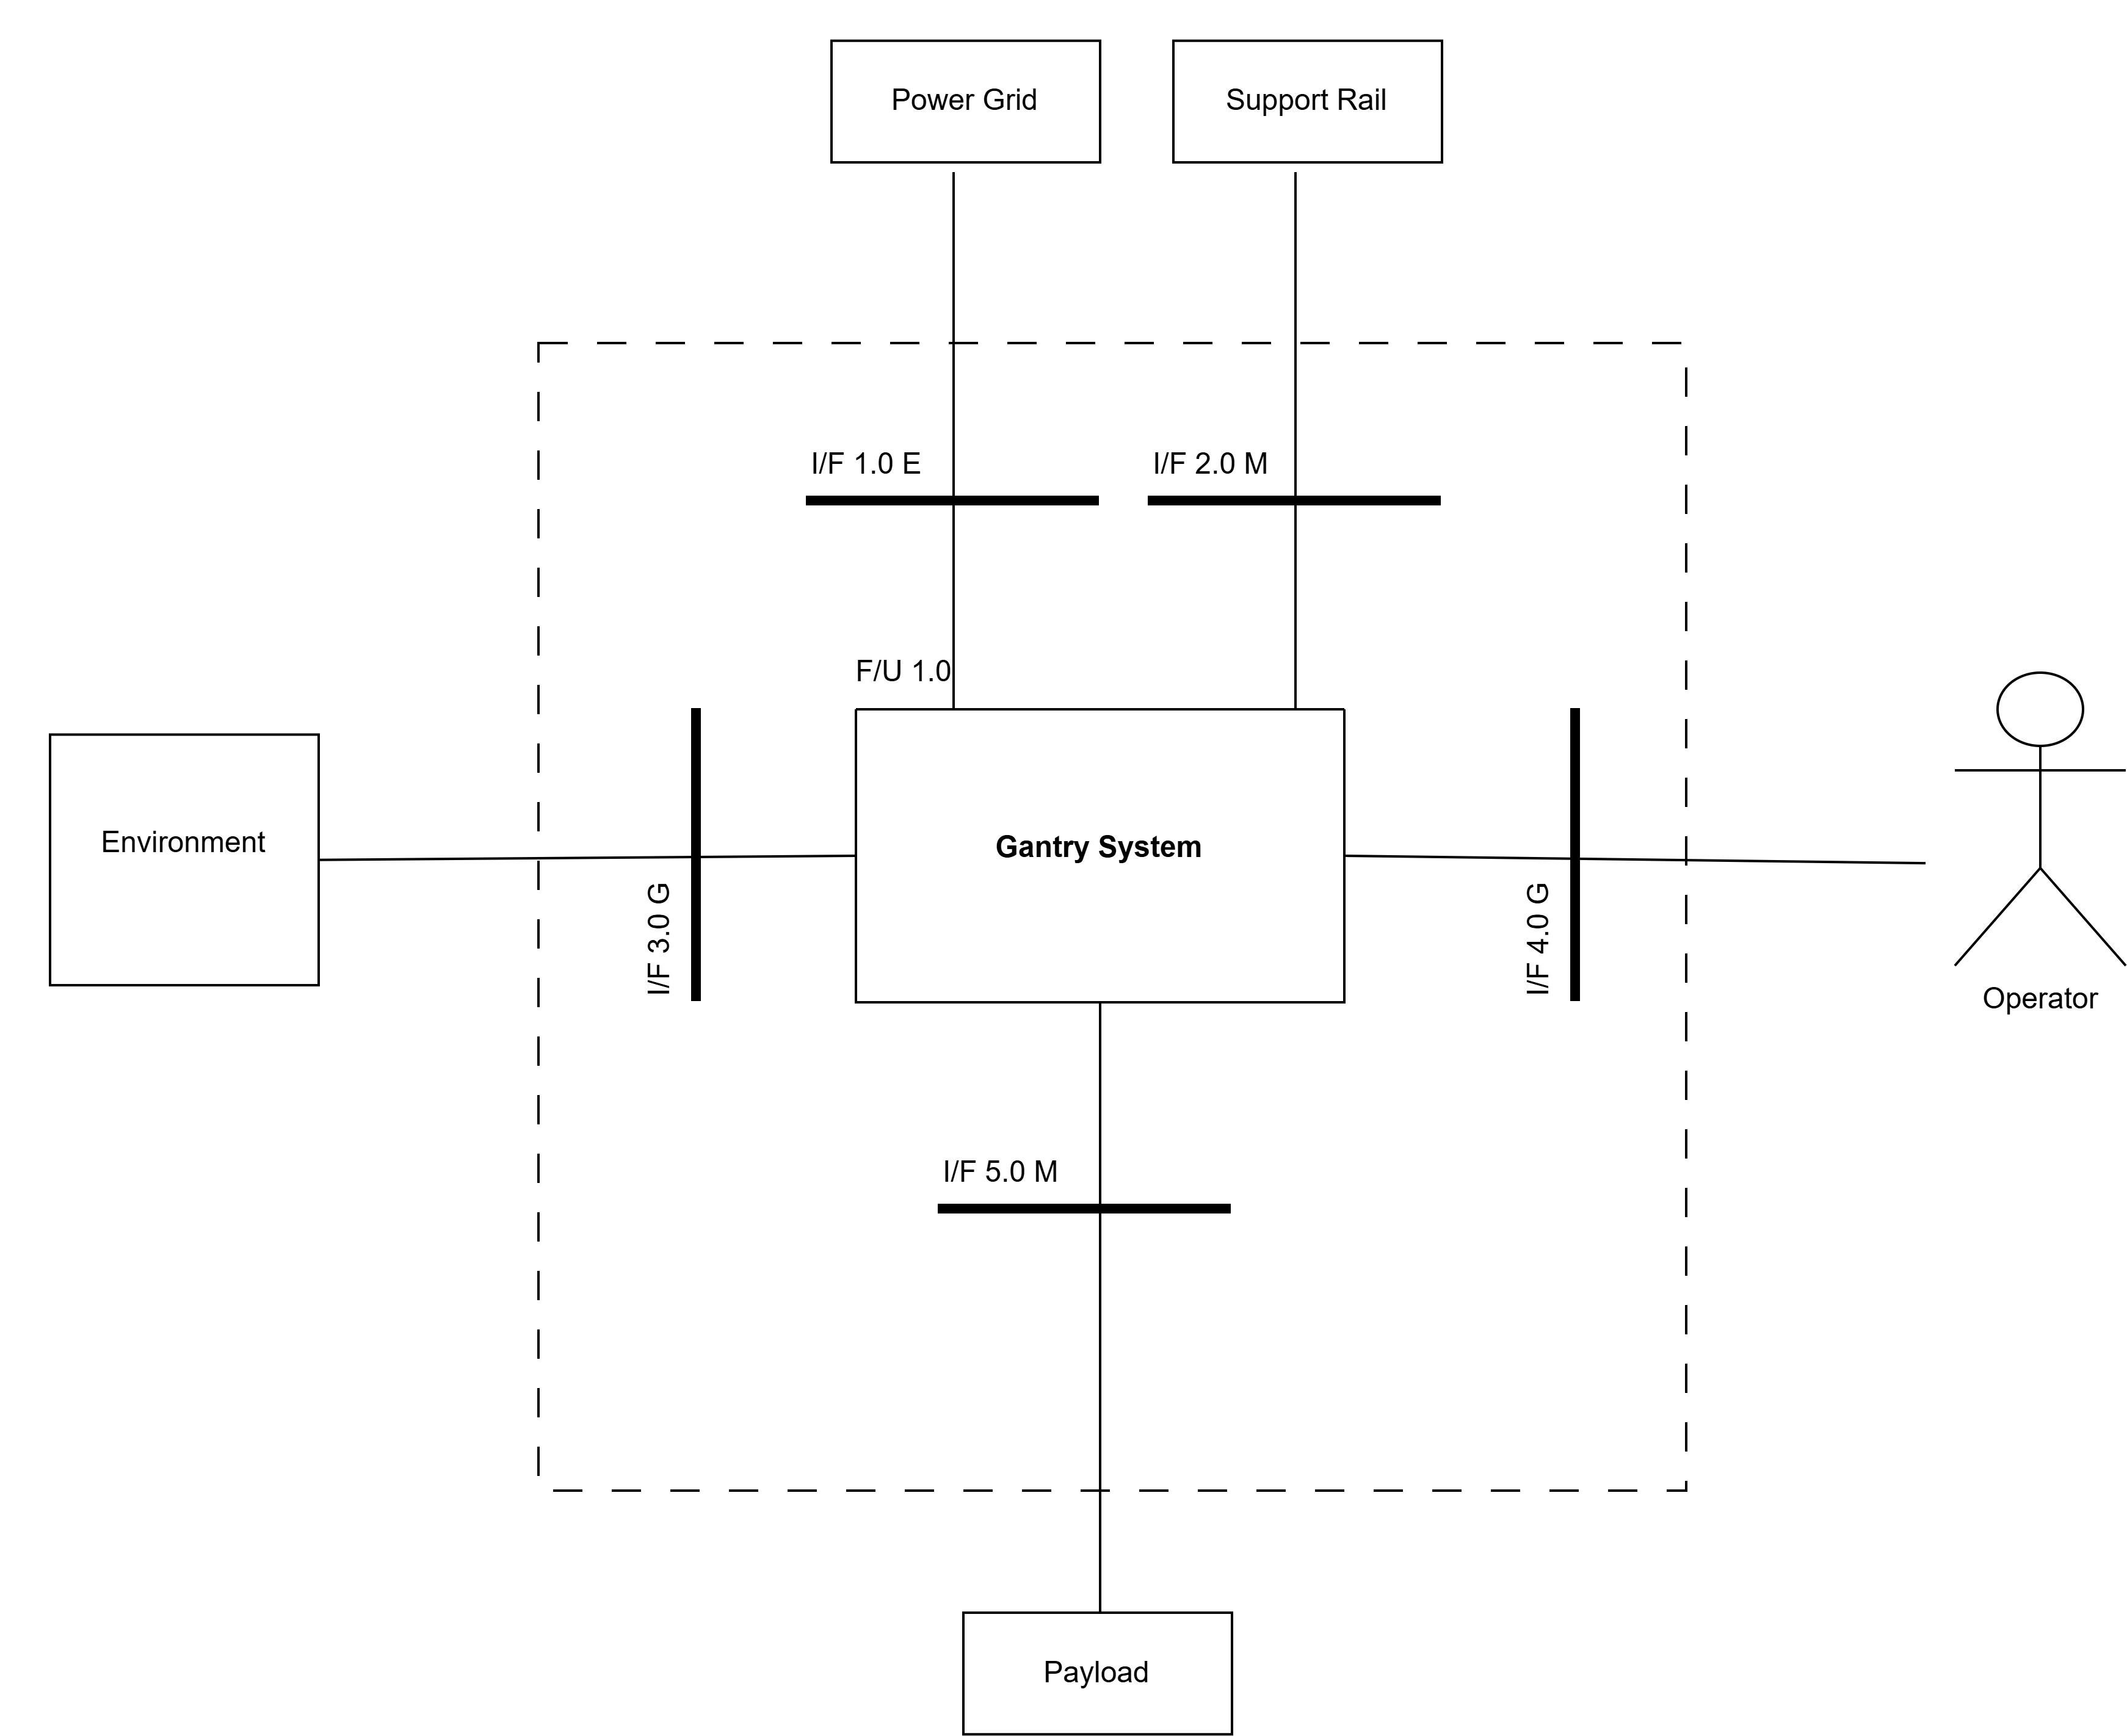
\includegraphics[width = \textwidth]{figures/Fig_Arch_Level0.png}
    \caption{System Architecture on Level 0}
    \label{fig:arch-level0}
\end{figure}

\subsection{Level 1: Gantry System F/U 1.0}
\label{subsec:gantry-system-fu}
The gantry system itself is divided up into five functional units as per the roles assigned to each group member as displayed in figure~\ref{fig:arch-level1}. Their subsequent interfaces and lower level functional units are covered by each member responsible.
\begin{figure}[H]
    \centering
    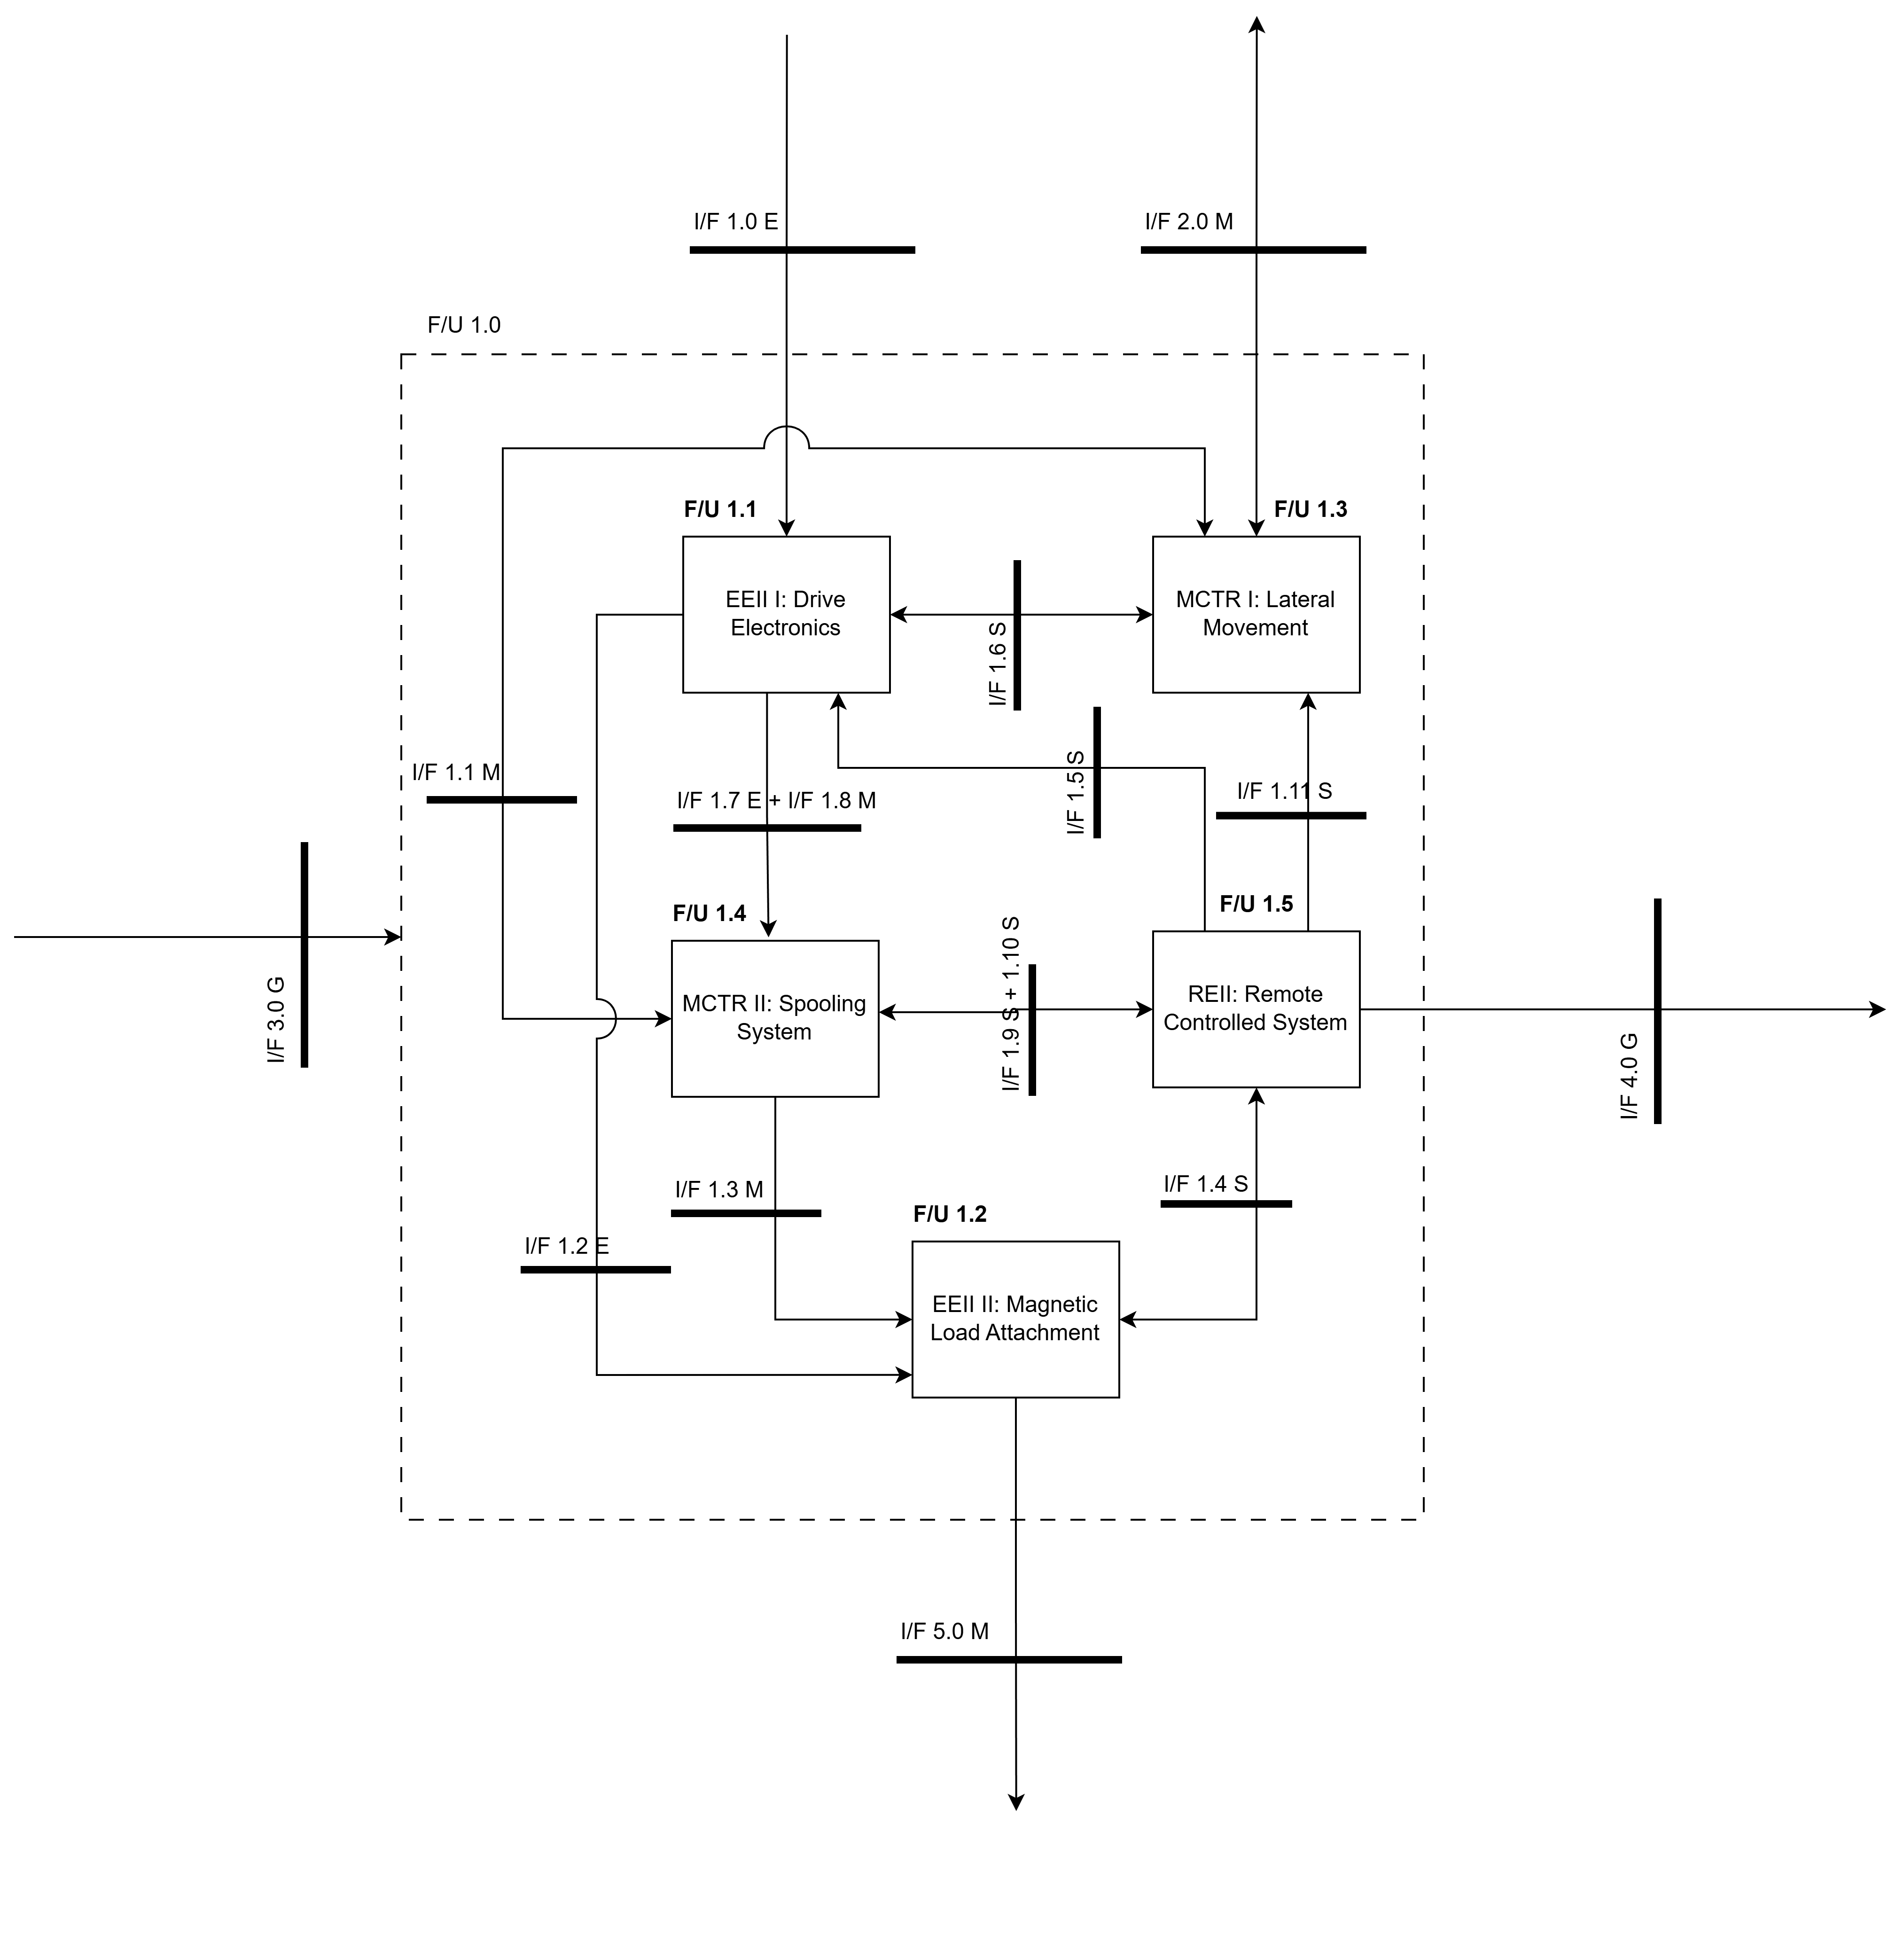
\includegraphics[width = \textwidth]{figures/Fig_Arch_Level1_GantrySystem.png}
    \caption{System Architecture on Level 1}
    \label{fig:arch-level1}
\end{figure}




\section{Level 2: Functional Units}
\label{sec:functional-units}
Each subsection handles one of the first level functional units introduced in section~\ref{sec:functional-units}.

\subsection{EERI I: Drive Electronics: F/U 1.1}
\label{subsec:eeri1-fu1p1}
EERI I Drive Electroncics by Jopie Roux.

The drive electronics subsystem converts the available single-phase 230VAC main supply to a 
controlled 3-phase supply for the induction motor. This interfaces with MCTR II through I/F 1.7 E
and 1.8 M. Figure~\ref{fig:arch-eeri1} shows the internal architecture of the subsystem and 
Table~\ref{tab:functional-units-eeri1} lists its three functional units. I additon to supplying them motor
EEII I is responsible for mains protection and distirubtion to the low voltage power supplies.
The subsystem also provides local protection against overcurrent and shoot-through conditions and
supplies current measurement feedback to the REII controller. The mains enter through I/F 1.0 E. 
The protected mains is supplied to the low voltage power supplies through I/F 1.2 E and 1.6 E. The
protected mains is also rectified and filtered to provide a DC bus for the inverter, which interfaces with
the induction motor through I/F 1.7 E. The motor interfaces mechanically with MCTR II through I/F 1.8 M.
Contorl commands are received form the REII controller through I/F 1.5 S through the isolation and gate
drivers. These control commands include the PWM signals used by the diver ICs to switch the IGBTs in the
inverter. The inverter also provides current feedback to the REII controller through I/F 1.5 S.


\begin{figure}[H]
    \centering
    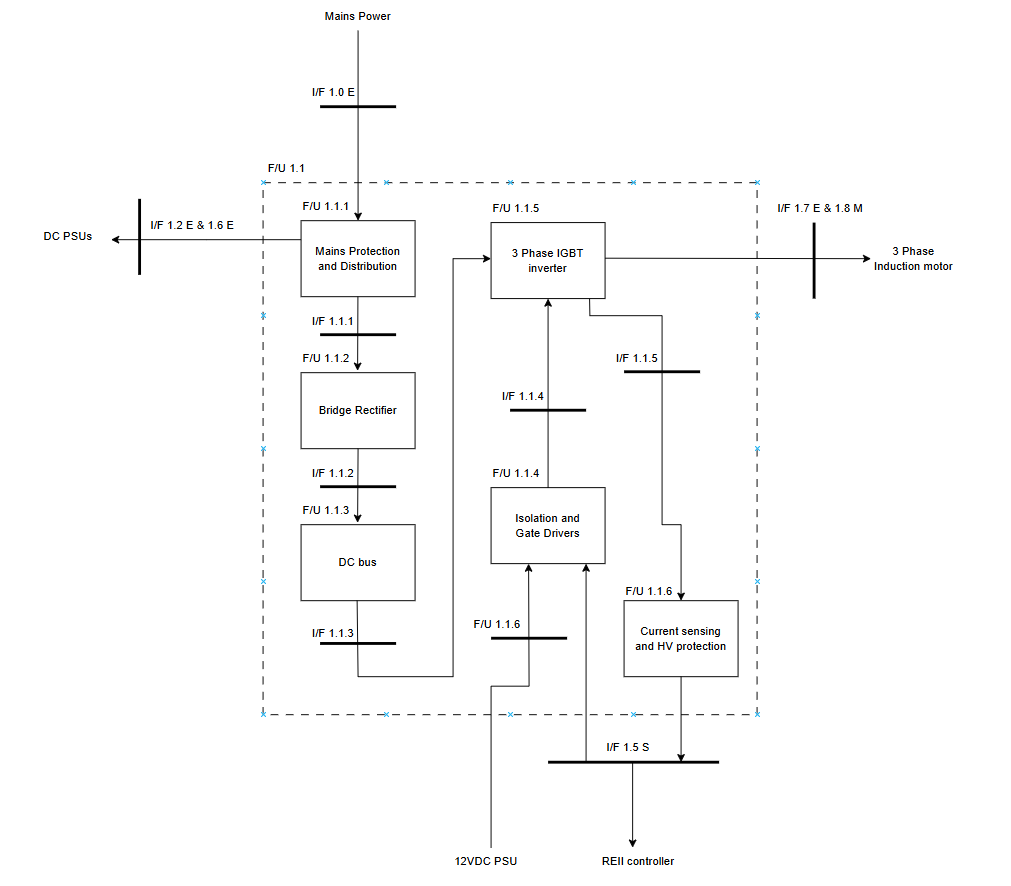
\includegraphics[width = \textwidth]{figures/Fig_Arch_Level2_EEII1.png}
    \caption{System Architecture of F/U 1.1 of the Drive Electronics Subsystem}
    \label{fig:arch-eeri1}
\end{figure}


\begin{table}[H]
    \centering
    \caption{Functional units of the EEII I drive electronics subsystem (F/U 1.1)}
    \label{tab:functional-units-eeri1}
    \begin{tabular}{@{} l l p{7cm} @{}}
        \toprule
        \textbf{F/U ID} & \textbf{Name} & \textbf{Description} \\
        \midrule
        F/U 1.1.1 & Mains Protection and Distribution
        & Receives the 230VAC mains supply and provides protected distribution to the low voltage 
        power supplies and drive electronics. This stage also contains the hardware isolation and emergency
        disconnect for high voltage applications. \\
        F/U 1.1.2 & Bridge Rectifier
         & Converts the 230VAC into a unregulated DC supply for the DC bus. \\
        F/U 1.1.3 & DC Bus
         & Smooths and stores the DC voltage for the inverter using a bulk capacitor. \\
        F/U 1.1.4 & Isolation and Gate Drivers
         & Provides electrical isolation between the REII controller and the high voltage drive electronics.
         The Driver ICs convert the incomming PWM signals into appropriate gate drive signals used to switch 
         the IGBTs in the inverter. \\
        F/U 1.1.5 & 3 Phase IGBT Inverter
         & Uses 6 IGBTs arranged in 3 half-bridges to convert DC to 3-phase AC. \\
        F/U 1.1.6 & Current sensing and HV Protection
         & Measures the drive current and provides the controller with a conditioned current feedback signal
         below 2.048V. \\
        \bottomrule
    \end{tabular}
\end{table}

\subsection{EERI II: Magnetic Load Attachment: F/U 1.2}
\label{subsec:eeri2-fu1p2}
The EERI II subsystem, engineered by J.P. Smith,
provides electromagnetic payload retention,
fast power switching and analog current sensing.
Figure~\ref{fig:arch-eeri2} shows the internal Level~2 architecture of the subsystem and its interface boundaries.
The subsystem decomposes into three lower-level functional units (Table~\ref{tab:eeri2-functional-units}).
The assembly is powered from the EEII~I $+13.5\,\text{V}$ DC bus via interface I/F~1.2~E, is suspended mechanically from the MCTR~II hoist cable hook via I/F~1.3~M,
and interfaces with the REII controller via I/F~1.10~S to receive PWM signal and transmit current signal ($V_{\mathrm{ISENSE}} \le 2.048\,\text{V}$).
The physical interface to the 20\,kg flat steel payload plate is designated as I/F~5.0~M.

\begin{figure}[H]
    \centering
    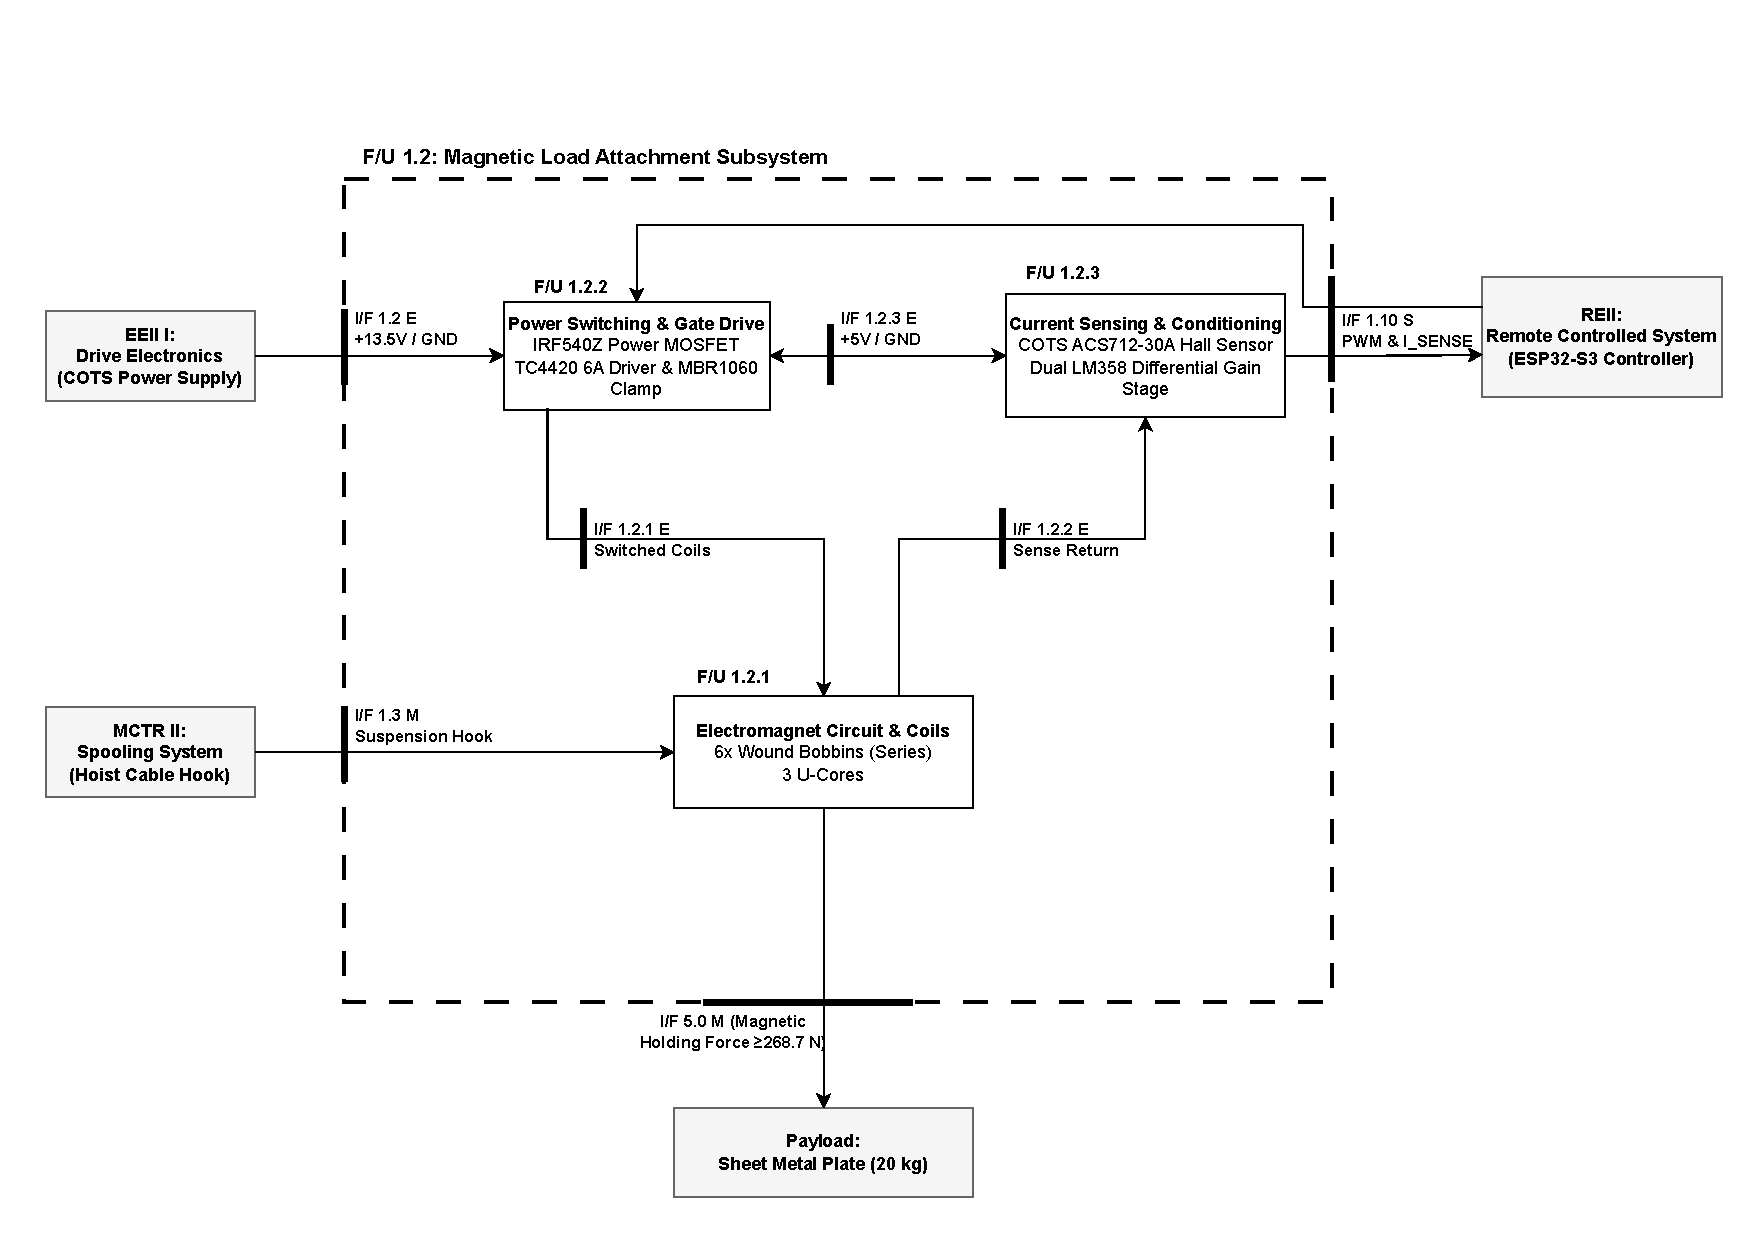
\includegraphics[width = \textwidth]{figures/JP_EEII_II_Subsystem.pdf}
    \caption{Level 2 architecture of the EERI II magnetic load attachment subsystem (F/U 1.2).}
    \label{fig:arch-eeri2}
\end{figure}

\begin{table}[H]
    \centering
    \caption{Functional units of the EERI II magnetic load attachment subsystem (F/U 1.2).}
    \label{tab:eeri2-functional-units}
    \begin{tabular}{@{} l l p{8.5cm} @{}}
        \toprule
        \textbf{F/U ID} & \textbf{Name} & \textbf{Description} \\
        \midrule
        F/U 1.2.1 & Magnetic Circuit \& Coils & Three U-core electromagnet assembly with six bobbins/legs ($28.0\,\text{m}$ of $1.00\,\text{mm}$ OD enamelled copper wire each, 286~turns/spool) providing $\ge 268.68\,\text{N}$ static holding capacity on $\ge 5\,\text{mm}$ steel plates (safety factor 1.37 on 20\,kg payload). \\
        F/U 1.2.2 & Power Switching  \& Gate Drive & High-current low-side switching using an IRF540Z  MOSFET driven by a TC4420 6\,A MOSFET driver from the $+13.5\,\text{V}$ rail, protected by an MBR1060 Schottky flyback diode. \\
        F/U 1.2.3 & Current Sensing  \& Conditioning & Galvanically isolated COTS ACS712-30A Hall-effect module conditioned via LM358 op-amp gain and offset subtraction, scaling $0\text{--}3\,\text{A}$ to $0.015\text{--}1.980\,\text{V} \le 2.048\,\text{V}$ for the REII ADC. \\
        \bottomrule
    \end{tabular}
\end{table}

\subsection{MCTR I: Lateral Movement: F/U 1.3}
\label{subsec:mctr1-fu1p3}
MCTR I Lateral Movement by Romeo Mapasa.
\begin{table}[H]
    \centering
    \caption{Operational Functional Units.}
    \label{tab:functional-units-mctr1}
    \begin{tabular}{@{} l l p{7cm} @{}}
        \toprule
        \textbf{F/U ID} & \textbf{Name} & \textbf{Description} \\
        \midrule
        F/U 1.0 & [Subsystem A] & [What this functional unit does.] \\
        F/U 2.0 & [Subsystem B] & [What this functional unit does.] \\
        F/U 3.0 & [Subsystem C] & [What this functional unit does.] \\
        \bottomrule
    \end{tabular}
\end{table}


\subsection{MCTR II: Spooling: F/U 1.4}
\label{subsec:mctr2-fu1p4}
MCTR II Spooling by Juan Fourie.
% =====================================================================
%  mctr2_parameters.tex  --  MCTR II (Spooling) parameter + calculation sheet
%
%  HOW TO USE
%   * Edit ONLY the \In... values in Section 1. Everything in Section 2
%     (\Raw... results) is computed from them by \fpeval, so every
%     table, equation and sentence that quotes a result updates on the
%     next compile.
%   * Units are noted per line. Torques in N.m unless stated.
%   * Display helpers:  \shown{Name}{digits}        -> number only
%                       \showv{Name}{digits}{unit}  -> number + unit
%   * This file is safe to \input from several chapters (loads once).
%   * Needs: LaTeX >= 2021 (\fpeval in kernel), amsmath, xcolor.
% =====================================================================
\ifdefined\MCTRIIparamsloaded\else
\def\MCTRIIparamsloaded{}

\providecommand{\tbd}[1]{\textcolor{red}{\textbf{[TBD: #1]}}}
\newcommand{\val}[2]{\ensuremath{#1\,\mathrm{#2}}}
\newcommand{\shown}[2]{\fpeval{round(\csname Raw#1\endcsname,#2)}}
\newcommand{\showv}[3]{\val{\fpeval{round(\csname Raw#1\endcsname,#2)}}{#3}}
% PASS/FAIL helpers: \passge{value}{limit} passes when value >= limit
\newcommand{\passge}[2]{\ifdim #1pt<#2pt \textcolor{red}{\textbf{FAIL}}\else\textcolor{green!45!black}{\textbf{PASS}}\fi}
\newcommand{\passle}[2]{\ifdim #1pt>#2pt \textcolor{red}{\textbf{FAIL}}\else\textcolor{green!45!black}{\textbf{PASS}}\fi}

% Functional-unit number of MCTR II (Level 1 drawing: F/U 1.4).
% NOTE: the Level 2 drawing currently labels sub-units 1.3.x; change the
% drawing to 1.4.x (or set this to 1.3 to match the drawing, but 1.3 is MCTR I).
\newcommand{\fuMII}{1.3}

% ---------------------------------------------------------------------
% 1. INPUTS  (edit these)
% ---------------------------------------------------------------------
% -- Loads, stroke, timing
\newcommand{\InMassRated}{20}    % kg   rated payload (PHY1)
\newcommand{\InMassDesign}{30}   % kg   design overload case (analysis only)
\newcommand{\InMassAttach}{2}    % kg   magnet + hook hanging on rope  [TBD: weigh]
\newcommand{\InGrav}{9.81}       % m/s^2
\newcommand{\InStroke}{1.6}      % m     hoist stroke (PT2)
\newcommand{\InTimeReq}{20}      % s     max stroke time (PT2)
\newcommand{\InServiceF}{1.5}    % -     service factor on drum torque
\newcommand{\InSFreq}{1.5}       % -     minimum acceptable safety factor (strength checks)
% -- Drum and rope
\newcommand{\InDrumD}{50}        % mm    drum core diameter (FROZEN; 70 mm entry removed)
\newcommand{\InDrumH}{60}        % mm    drum usable length
\newcommand{\InRopeD}{5}         % mm    rope diameter
\newcommand{\InRopeCentre}{1}    % 1 = tension acts at rope centre-line (D+d); 0 = old spreadsheet (D only)
% -- Motor and VSD
\newcommand{\InMotorP}{180}      % W     Askari MS632-4
\newcommand{\InMotorN}{1360}     % rpm   at rated frequency
\newcommand{\InMotorF}{50}       % Hz    rated frequency
\newcommand{\InVsdF}{50}         % Hz    frequency VSD will actually deliver  [TBD: EEII I to confirm]
% -- Gearbox (stage A = motor side, stage B = drum side)
\newcommand{\InNpA}{16}   \newcommand{\InNgA}{102}   % pinion / gear teeth, stage A
\newcommand{\InNpB}{16}   \newcommand{\InNgB}{102}   % pinion / gear teeth, stage B
\newcommand{\InModA}{1.5} \newcommand{\InModB}{2}    % mm module
\newcommand{\InFwA}{10}   \newcommand{\InFwB}{15}    % mm face width
\newcommand{\InPhi}{25}          % deg   pressure angle (use 24 if Inventor forces it; both gears of a mesh must match)
\newcommand{\InYpA}{0.296}       % Lewis form factor, pinion  (Shigley Tbl 14-2, 20 deg value: conservative for 25 deg)
\newcommand{\InYgA}{0.447}       % Lewis form factor, gear
\newcommand{\InYpB}{0.296}
\newcommand{\InYgB}{0.447}
\newcommand{\InEta}{0.95}        % -     efficiency per gear stage
\newcommand{\InSigAllow}{20}     % MPa   allowable PETG root stress [GUESS: replace with printed-coupon result / SF]
\newcommand{\InClear}{0.25}      % mm    added centre-distance clearance (printed backlash)
\newcommand{\InBed}{220}         % mm    print bed edge length [TBD: confirm printer]
% -- Shaft, hub and fastener
\newcommand{\InShaftD}{10}       % mm    shaft diameter
\newcommand{\InSpan}{100}        % mm    bearing span (centre-to-centre)
\newcommand{\InKt}{2}            % -     bending stress-concentration factor, cross-hole
\newcommand{\InKts}{2}           % -     torsion stress-concentration factor, cross-hole
\newcommand{\InSy}{250}          % MPa   yield strength  [TBD: replace with certified grade, e.g. EN8 bright bar]
\newcommand{\InBoltD}{4}         % mm    cross-bolt diameter
\newcommand{\InHubWall}{8}       % mm    hub wall length bearing on bolt
\newcommand{\InHubAllow}{20}     % MPa   allowable PETG bearing stress [GUESS]
% -- Brake
\newcommand{\InBrakeSF}{2}       % -     brake torque safety factor
\newcommand{\InBrakeRated}{0}    % N.m   datasheet holding torque; 0 = not yet known  [TBD: datasheet]
% -- Load cell and HX711
\newcommand{\InCellCap}{100}     % kg    YZC-516 rated capacity
\newcommand{\InCellSens}{2}      % mV/V  rated output [TBD: datasheet]
\newcommand{\InExc}{5}           % V     excitation (HX711 supply)
\newcommand{\InGain}{128}        % -     HX711 channel A gain
\newcommand{\InSps}{80}          % SPS   HX711 output rate (RATE pin high)
\newcommand{\InFilt}{4}          % -     samples averaged by interlock filter
\newcommand{\InNoise}{500}       % counts peak-to-peak noise [GUESS: measure with motor running]
\newcommand{\InTrip}{1.25}       % -     overload trip as multiple of (rated + attachment)
% -- Cost (R, incl. VAT and shipping, from Cost_and_Budget.xlsx)
\newcommand{\InBudget}{5000}
\newcommand{\InCostBearings}{116.24}
\newcommand{\InCostCell}{429.00}     % [CHECK: sheet unit 493.35 + 135.70 shipping = 629.05]
\newcommand{\InCostHX}{179.40}       % [CHECK: unit price 43.70]
\newcommand{\InCostPSU}{390.17}
\newcommand{\InCostBrake}{907.68}    % excluded from the sheet's own subtotal

% ---------------------------------------------------------------------
% 2. DERIVED RESULTS  (do not edit)
% ---------------------------------------------------------------------
% -- Kinematics
\newcommand{\RawDeff}{\fpeval{\InDrumD+\InRopeCentre*\InRopeD}}
\newcommand{\RawVreq}{\fpeval{\InStroke*1000/\InTimeReq}}
\newcommand{\RawWraps}{\fpeval{\InStroke*1000/(pi*\RawDeff)}}
\newcommand{\RawWrapsFit}{\fpeval{floor(\InDrumH/\InRopeD)}}
\newcommand{\RawiA}{\fpeval{\InNgA/\InNpA}}
\newcommand{\RawiB}{\fpeval{\InNgB/\InNpB}}
\newcommand{\RawiT}{\fpeval{\RawiA*\RawiB}}
\newcommand{\RawNmot}{\fpeval{\InMotorN*\InVsdF/\InMotorF}}
\newcommand{\RawNdrum}{\fpeval{\RawNmot/\RawiT}}
\newcommand{\RawVline}{\fpeval{pi*\RawDeff*\RawNdrum/60}}
\newcommand{\RawTstroke}{\fpeval{\InStroke*1000/\RawVline}}
\newcommand{\RawSpeedMargin}{\fpeval{(\RawVline/\RawVreq-1)*100}}
\newcommand{\RawiReq}{\fpeval{pi*\RawDeff*\RawNmot/(60*\RawVreq)}}
\newcommand{\RawFmin}{\fpeval{\RawVreq*60*\RawiT/(pi*\RawDeff)*\InMotorF/\InMotorN}}
% -- Drum torque, motor sizing
\newcommand{\RawFropeR}{\fpeval{\InMassRated*\InGrav}}
\newcommand{\RawFropeD}{\fpeval{\InMassDesign*\InGrav}}
\newcommand{\RawTdrR}{\fpeval{\InMassRated*\InGrav*\RawDeff/2000}}
\newcommand{\RawTdrD}{\fpeval{\InMassDesign*\InGrav*\RawDeff/2000*\InServiceF}}
\newcommand{\RawTdrSheet}{\fpeval{\InMassDesign*\InGrav*\InDrumD/2000*\InServiceF}}
\newcommand{\RawEtaGB}{\fpeval{\InEta*\InEta}}
\newcommand{\RawTmReq}{\fpeval{\RawTdrR/(\RawiT*\RawEtaGB)}}
\newcommand{\RawTmRated}{\fpeval{\InMotorP/(2*pi*\InMotorN/60)}}
\newcommand{\RawTmMargin}{\fpeval{\RawTmRated/\RawTmReq}}
\newcommand{\RawPmech}{\fpeval{\InMassRated*\InGrav*\RawVline/1000/\RawEtaGB}}
\newcommand{\RawPavail}{\fpeval{\InMotorP*\InVsdF/\InMotorF}}
% -- Gear loads (design case) and Lewis stress
\newcommand{\RawTtwo}{\fpeval{\RawTdrD/(\RawiB*\InEta)}}
\newcommand{\RawTone}{\fpeval{\RawTtwo/(\RawiA*\InEta)}}
\newcommand{\RawFtB}{\fpeval{2*\RawTtwo*1000/(\InModB*\InNpB)}}
\newcommand{\RawFtA}{\fpeval{2*\RawTone*1000/(\InModA*\InNpA)}}
\newcommand{\RawFnB}{\fpeval{\RawFtB/cosd(\InPhi)}}
\newcommand{\RawFnA}{\fpeval{\RawFtA/cosd(\InPhi)}}
\newcommand{\RawFrB}{\fpeval{\RawFtB*tand(\InPhi)}}
\newcommand{\RawSigPA}{\fpeval{\RawFtA/(\InFwA*\InModA*\InYpA)}}
\newcommand{\RawSigGA}{\fpeval{\RawFtA/(\InFwA*\InModA*\InYgA)}}
\newcommand{\RawSigPB}{\fpeval{\RawFtB/(\InFwB*\InModB*\InYpB)}}
\newcommand{\RawSigGB}{\fpeval{\RawFtB/(\InFwB*\InModB*\InYgB)}}
\newcommand{\RawSFpA}{\fpeval{\InSigAllow/\RawSigPA}}
\newcommand{\RawSFpB}{\fpeval{\InSigAllow/\RawSigPB}}
% -- Gear geometry
\newcommand{\RawDpinA}{\fpeval{\InModA*\InNpA}}
\newcommand{\RawDgearA}{\fpeval{\InModA*\InNgA}}
\newcommand{\RawDpinB}{\fpeval{\InModB*\InNpB}}
\newcommand{\RawDgearB}{\fpeval{\InModB*\InNgB}}
\newcommand{\RawDoGearA}{\fpeval{\InModA*(\InNgA+2)}}
\newcommand{\RawDoGearB}{\fpeval{\InModB*(\InNgB+2)}}
\newcommand{\RawCdA}{\fpeval{\InModA*(\InNpA+\InNgA)/2+\InClear}}
\newcommand{\RawCdB}{\fpeval{\InModB*(\InNpB+\InNgB)/2+\InClear}}
\newcommand{\RawZmin}{\fpeval{2/(sind(\InPhi)^2)}}
\newcommand{\RawDbPinB}{\fpeval{\RawDpinB*cosd(\InPhi)}}
\newcommand{\RawBedUse}{\fpeval{max(\RawDoGearA,\RawDoGearB)/\InBed*100}}
% -- Shaft (macros with arguments: #1 = payload mass kg, #2 = torque factor)
\newcommand{\Tdr}[2]{\fpeval{#1*\InGrav*\RawDeff/2*#2}}                                   % N.mm
\newcommand{\FgB}[2]{\fpeval{2*\Tdr{#1}{#2}/(\InEta*\InModB*\InNgB*cosd(\InPhi))}}        % N
\newcommand{\Msh}[2]{\fpeval{(#1*\InGrav+\FgB{#1}{#2})*\InSpan/4}}                        % N.mm
\newcommand{\SigBsh}[2]{\fpeval{32*\Msh{#1}{#2}/(pi*\InShaftD^3)}}                        % MPa
\newcommand{\Taush}[2]{\fpeval{16*\Tdr{#1}{#2}/(pi*\InShaftD^3)}}                         % MPa
\newcommand{\VMsh}[2]{\fpeval{sqrt((\InKt*\SigBsh{#1}{#2})^2+3*(\InKts*\Taush{#1}{#2})^2)}} % MPa
\newcommand{\RawFgD}{\FgB{\InMassDesign}{\InServiceF}}
\newcommand{\RawMshD}{\Msh{\InMassDesign}{\InServiceF}}
\newcommand{\RawSigBD}{\SigBsh{\InMassDesign}{\InServiceF}}
\newcommand{\RawTauD}{\Taush{\InMassDesign}{\InServiceF}}
\newcommand{\RawVMD}{\VMsh{\InMassDesign}{\InServiceF}}
\newcommand{\RawVMR}{\VMsh{\InMassRated}{1}}
\newcommand{\RawSFsD}{\fpeval{\InSy/\RawVMD}}
\newcommand{\RawSFsR}{\fpeval{\InSy/\RawVMR}}
% -- Hub / cross-bolt (design case, drum shaft)
\newcommand{\RawFside}{\fpeval{\RawTdrD*1000/\InShaftD}}
\newcommand{\RawSigHub}{\fpeval{\RawFside/(\InBoltD*\InHubWall)}}
\newcommand{\RawTauBolt}{\fpeval{\RawFside/(pi*\InBoltD^2/4)}}
\newcommand{\RawSFhub}{\fpeval{\InHubAllow/\RawSigHub}}
% -- Rated-case (20 kg, no service factor) checks for gears and hub
\newcommand{\RawLoadRatio}{\fpeval{\RawTdrR/\RawTdrD}}
\newcommand{\RawSFpAR}{\fpeval{\RawSFpA/\RawLoadRatio}}
\newcommand{\RawSFpBR}{\fpeval{\RawSFpB/\RawLoadRatio}}
\newcommand{\RawSigHubR}{\fpeval{\RawSigHub*\RawLoadRatio}}
\newcommand{\RawSFhubR}{\fpeval{\InHubAllow/\RawSigHubR}}
% -- Brake
\newcommand{\RawTholdDrum}{\fpeval{\InMassDesign*\InGrav*\RawDeff/2000}}
\newcommand{\RawTholdIn}{\fpeval{\RawTholdDrum/\RawiT}}
\newcommand{\RawBrakeReqDrum}{\fpeval{\RawTholdDrum*\InBrakeSF}}
\newcommand{\RawBrakeReqIn}{\fpeval{\RawTholdIn*\InBrakeSF}}
\newcommand{\BrakeMarginIn}{\ifdim\InBrakeRated pt=0pt\tbd{datasheet torque}\else\fpeval{round(\InBrakeRated/\RawBrakeReqIn,1)}\fi}
\newcommand{\BrakeMarginDrum}{\ifdim\InBrakeRated pt=0pt\tbd{datasheet torque}\else\fpeval{round(\InBrakeRated/\RawBrakeReqDrum,1)}\fi}
% -- Load cell and HX711
\newcommand{\RawFcell}{\fpeval{(\InMassRated+\InMassAttach)*\InGrav}}
\newcommand{\RawMtrip}{\fpeval{(\InMassRated+\InMassAttach)*\InTrip}}
\newcommand{\RawCellUse}{\fpeval{\RawMtrip/\InCellCap*100}}
\newcommand{\RawSigFS}{\fpeval{\InCellSens*\InExc}}
\newcommand{\RawAdcRange}{\fpeval{0.5*\InExc/\InGain*1000}}
\newcommand{\RawCntPerKg}{\fpeval{\InCellSens/1000/\InCellCap*\InGain/0.5*2^23}}
\newcommand{\RawResG}{\fpeval{\InNoise/\RawCntPerKg*1000}}
\newcommand{\RawLatency}{\fpeval{\InFilt/\InSps*1000}}
\newcommand{\RawTravel}{\fpeval{\RawVline*\RawLatency/1000}}
% -- Cost
\newcommand{\RawCostTot}{\fpeval{\InCostBearings+\InCostCell+\InCostHX+\InCostPSU+\InCostBrake}}
\newcommand{\RawBudgetLeft}{\fpeval{\InBudget-\RawCostTot}}
\newcommand{\RawBudgetUse}{\fpeval{\RawCostTot/\InBudget*100}}
\fi

The spooling subsystem raises and lowers the payload on a rope wound onto a
drum, holds it safely when unpowered, and reports the on-hook load to the
controller. Figure~\ref{fig:arch-mctr2} shows its internal architecture and
Table~\ref{tab:fu-mctr2} lists its six functional units. The induction motor
that drives the gearbox is supplied and powered by EEII~I and enters this
subsystem through interface I/F~1.7~E and I/F~1.8~M. The gearbox and spool itself is mounted to the frame of MCTR~I through I/F~1.1~M. The brake signal is received from REII through I/F~1.9~S and the load cell telemetry with the power and ground required by the HX711 is sent and received by REII through I/F~1.10~S. EERI~II has its electromagnet and electrical/signal wiring connected through I/F~1.3~M.
(Chapter~\ref{ch:interface-control}).

\begin{figure}[H]
    \centering
    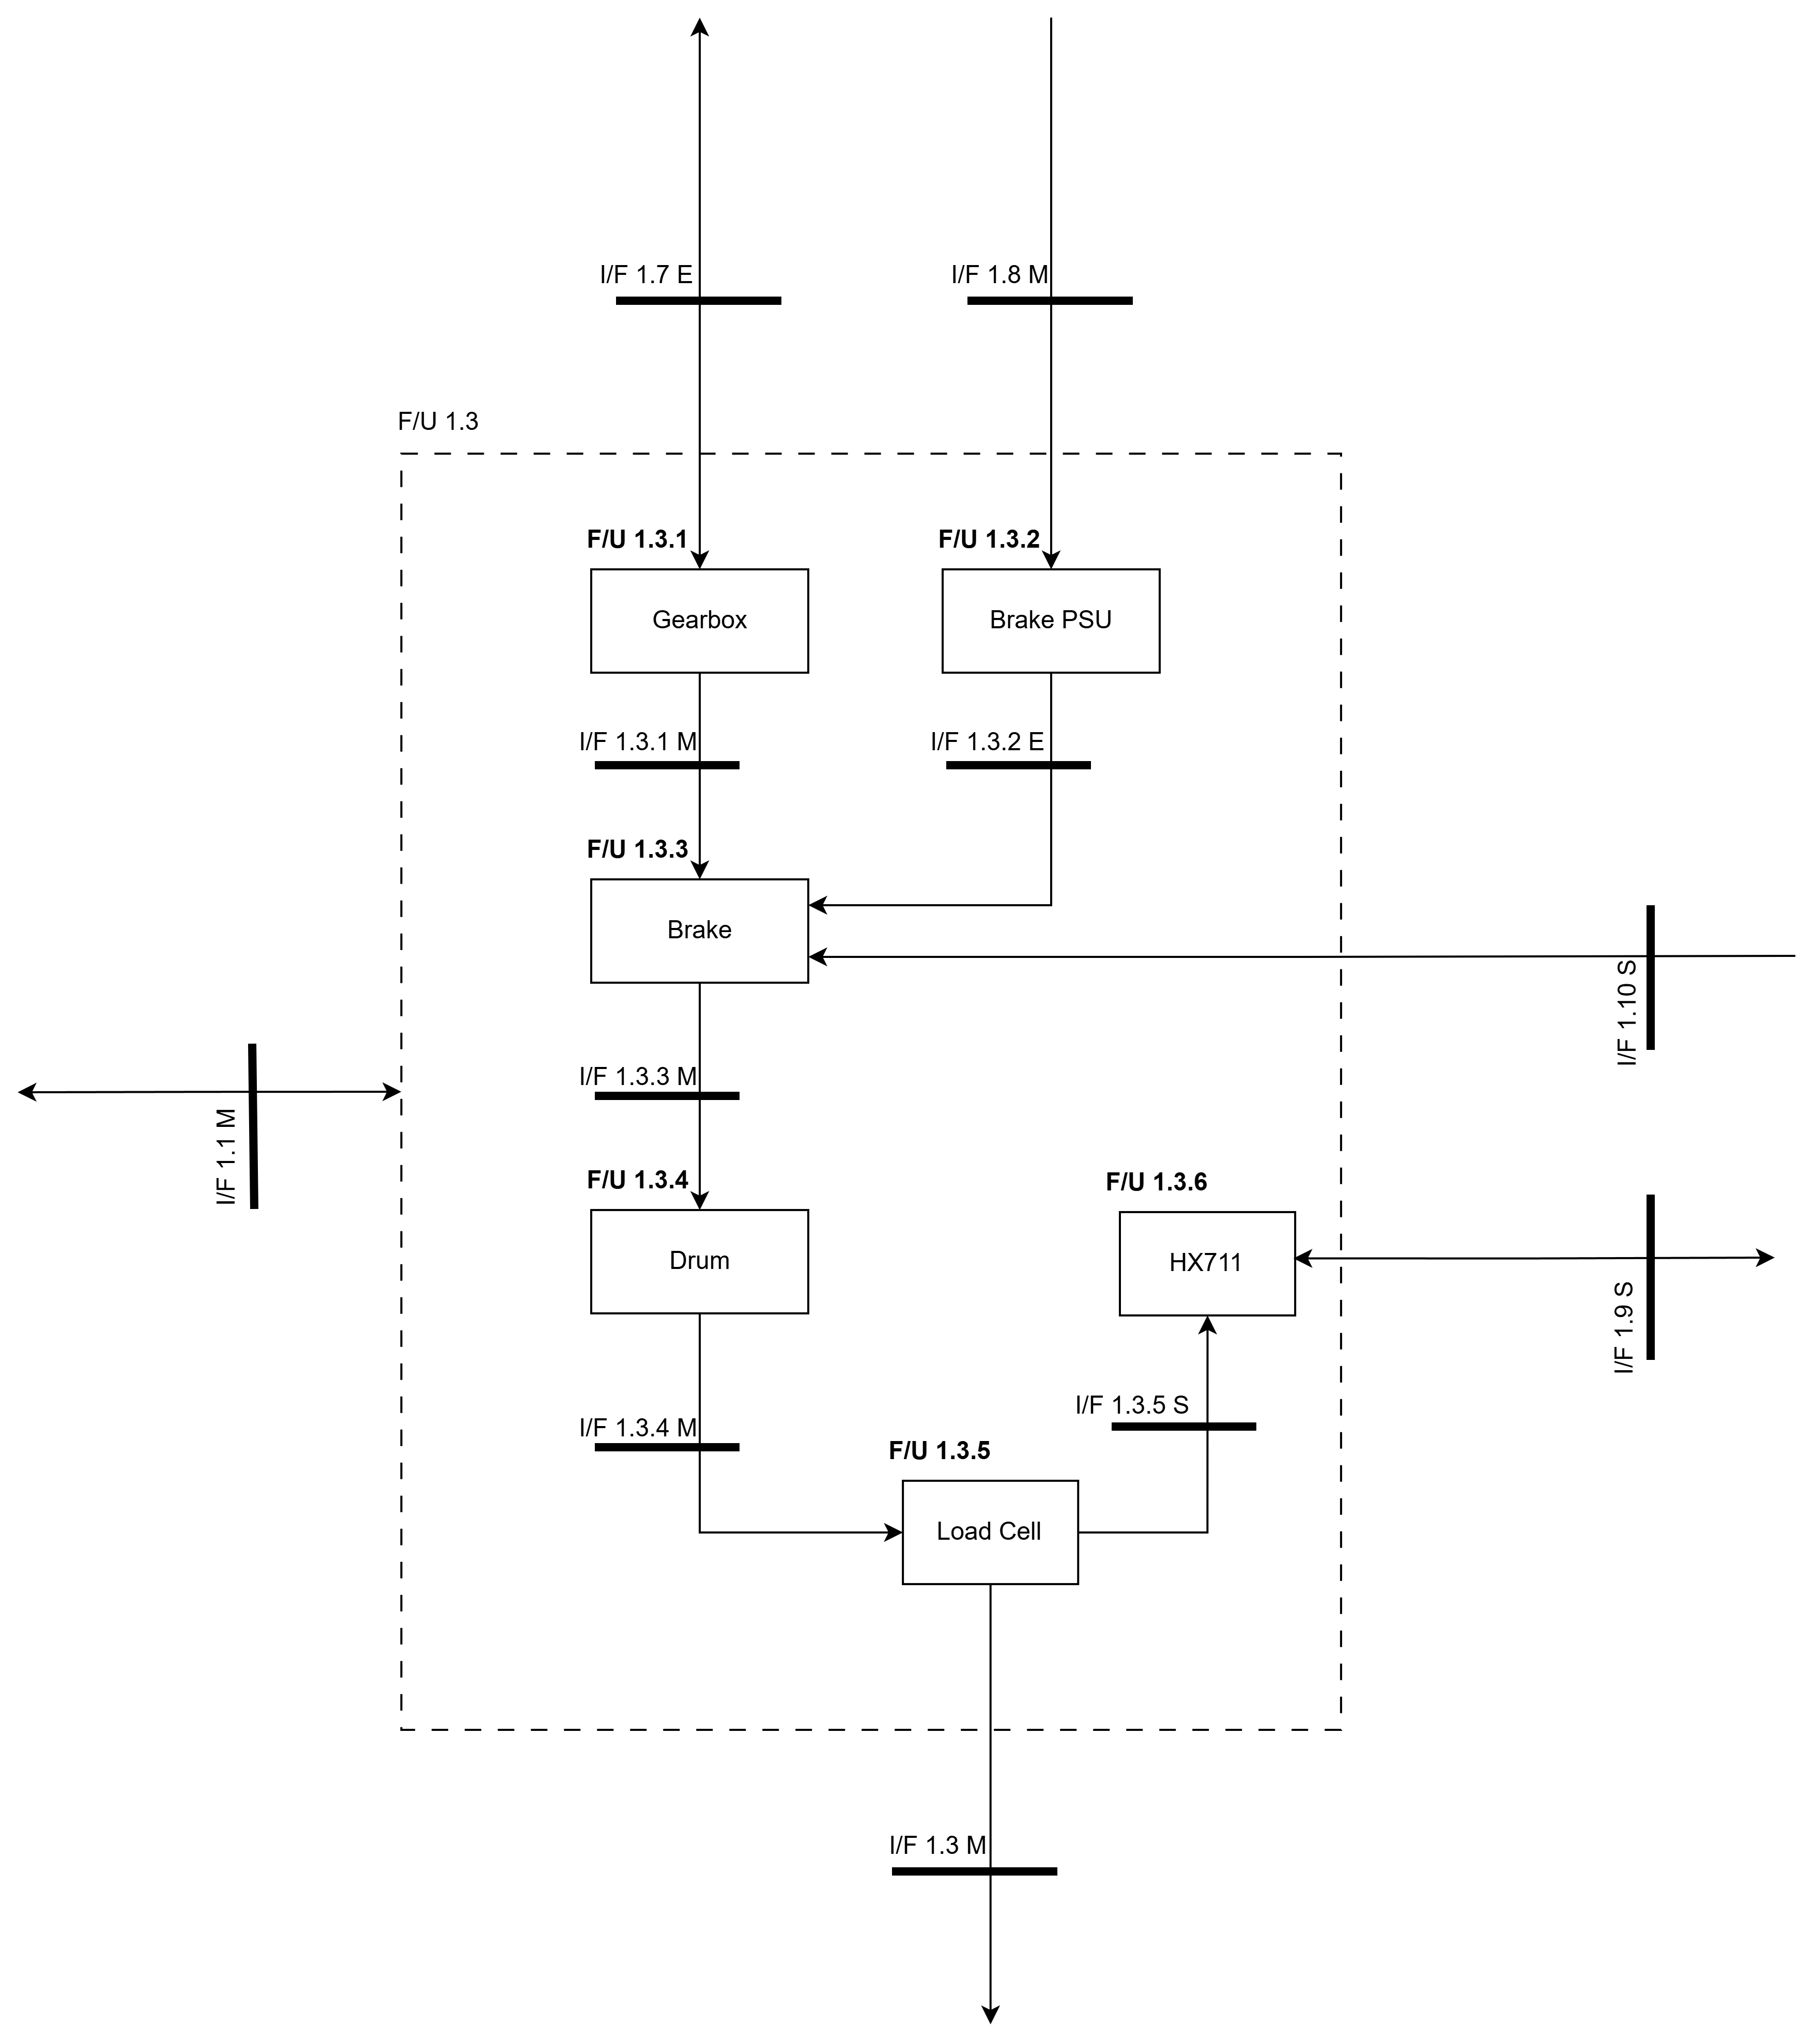
\includegraphics[width = \textwidth]{figures/Fig_Arch_Level2_MCTRII.png}
    \caption{System Architecture of F/U 1.4 of the Spooling Subsystem}
    \label{fig:arch-mctr2}
\end{figure}

\begin{table}[H]
    \centering
      \caption{Functional units of the MCTR II spooling subsystem (F/U \fuMII).}
    \label{tab:fu-mctr2}
    \small
    \begin{tabularx}{\textwidth}{@{} l l X @{}}
        \toprule
        \textbf{F/U ID} & \textbf{Name} & \textbf{Description} \\
        \midrule
        F/U \fuMII.1 & Gearbox &
            Two-stage compound spur gearbox (3D-printed PETG, no worm gear,
            DR2). Reduces motor speed (\showv{Nmot}{0}{rpm}) by an overall
            ratio of \shown{iT}{2}:1 to \showv{Ndrum}{1}{rpm} at the drum and
            multiplies motor torque to \showv{TdrR}{2}{N\,m} (rated load). \\
        F/U \fuMII.2 & Brake PSU &
            Stand-alone 48\,V DC supply for the brake coil, fed from the
            mains distribution provided by EEII~I. Switched through a relay
            that defaults to the de-energised state. \\
        F/U \fuMII.3 & Brake &
            Spring-applied, electrically released holding brake. Engages
            automatically on loss of power or command and holds the payload
            without drift (FR6). \\
        F/U \fuMII.4 & Drum &
            \InDrumD\,mm drum carrying \InRopeD\,mm rope in a single layer
            (\shown{Wraps}{1} wraps for the \InStroke\,m stroke, capacity
            \shown{WrapsFit}{0} wraps). Output shaft of the gearbox drives it
            through a hub with a cross-bolt. \\
        F/U \fuMII.5 & Load cell &
            S-type load cell (\InCellCap\,kg) carrying a sheave through which
            the rope passes; measures the on-hook load for telemetry and
            overload interlock (FR5). \\
        F/U \fuMII.6 & HX711 &
            24-bit bridge ADC converting the load-cell signal to a 2-wire
            digital stream (\InSps\,SPS) for the controller. \\
        \bottomrule
    \end{tabularx}
\end{table}

\subsection{REII: Remote Control Dashboard: F/U 1.5}
\label{subsec:reii-fu1p5}
REII Remote Control Dashboard by Anton Swanepoel

The proposed REII subsystem would provide crane commands and display
lateral position, speed, load, current, fault and the current grip status.
Figure~\ref{fig:reii-architecture} shows the architecture;
Table~\ref{tab:functional-units-reii} lists five functional units.
Commands would pass from the Python dashboard through the STM32 UART
ground station and nRF24 radios to the ESP32-S3; telemetry would return
along this path. \cite{nwu_sysrs2026,nwu_reii_scope2026}

I/F~1.5.4 would link the controller to EERI~I's inverter, while
I/F~1.5.5 would connect it to EERI~II's magnet. Both would return
current feedback for fault or grip inference. MCTR~I would receive
lateral commands and return encoder feedback through I/F~1.5.6.
Through I/F~1.5.7, REII would command MCTR~II's brake, power the HX711,
drive SCK and read DAT. Chapter~\ref{ch:interface-control} details these
interfaces. Final integration remains incomplete.
\cite{nwu_sysrs2026,nwu_reii_scope2026,nwu_s3_board2026}

\begin{table}[H]
    \centering
    \caption{Operational functional units of REII.}
    \label{tab:functional-units-reii}
    \begin{tabularx}{\textwidth}{@{}
        l
        >{\raggedright\arraybackslash}p{4cm}
        >{\raggedright\arraybackslash}X
    @{}}
        \toprule
        \textbf{F/U ID} & \textbf{Name} & \textbf{Description} \\
        \midrule
        F/U~1.5.1 & Python dashboard &
        Accept operator commands and display telemetry and faults. \\

        F/U~1.5.2 & STM32 ground station &
        Transfer messages between the PC serial connection and the radio. \\

        F/U~1.5.3 & Ground radio &
        Send commands and receive controller replies. \\

        F/U~1.5.4 & Hoist radio &
        Receive commands and return results and telemetry. \\

        F/U~1.5.5 & ESP32-S3 controller &
        Check requests, generate control outputs and collect subsystem data. \\
        \bottomrule
    \end{tabularx}
\end{table}

\begin{figure}[H]
    \centering
    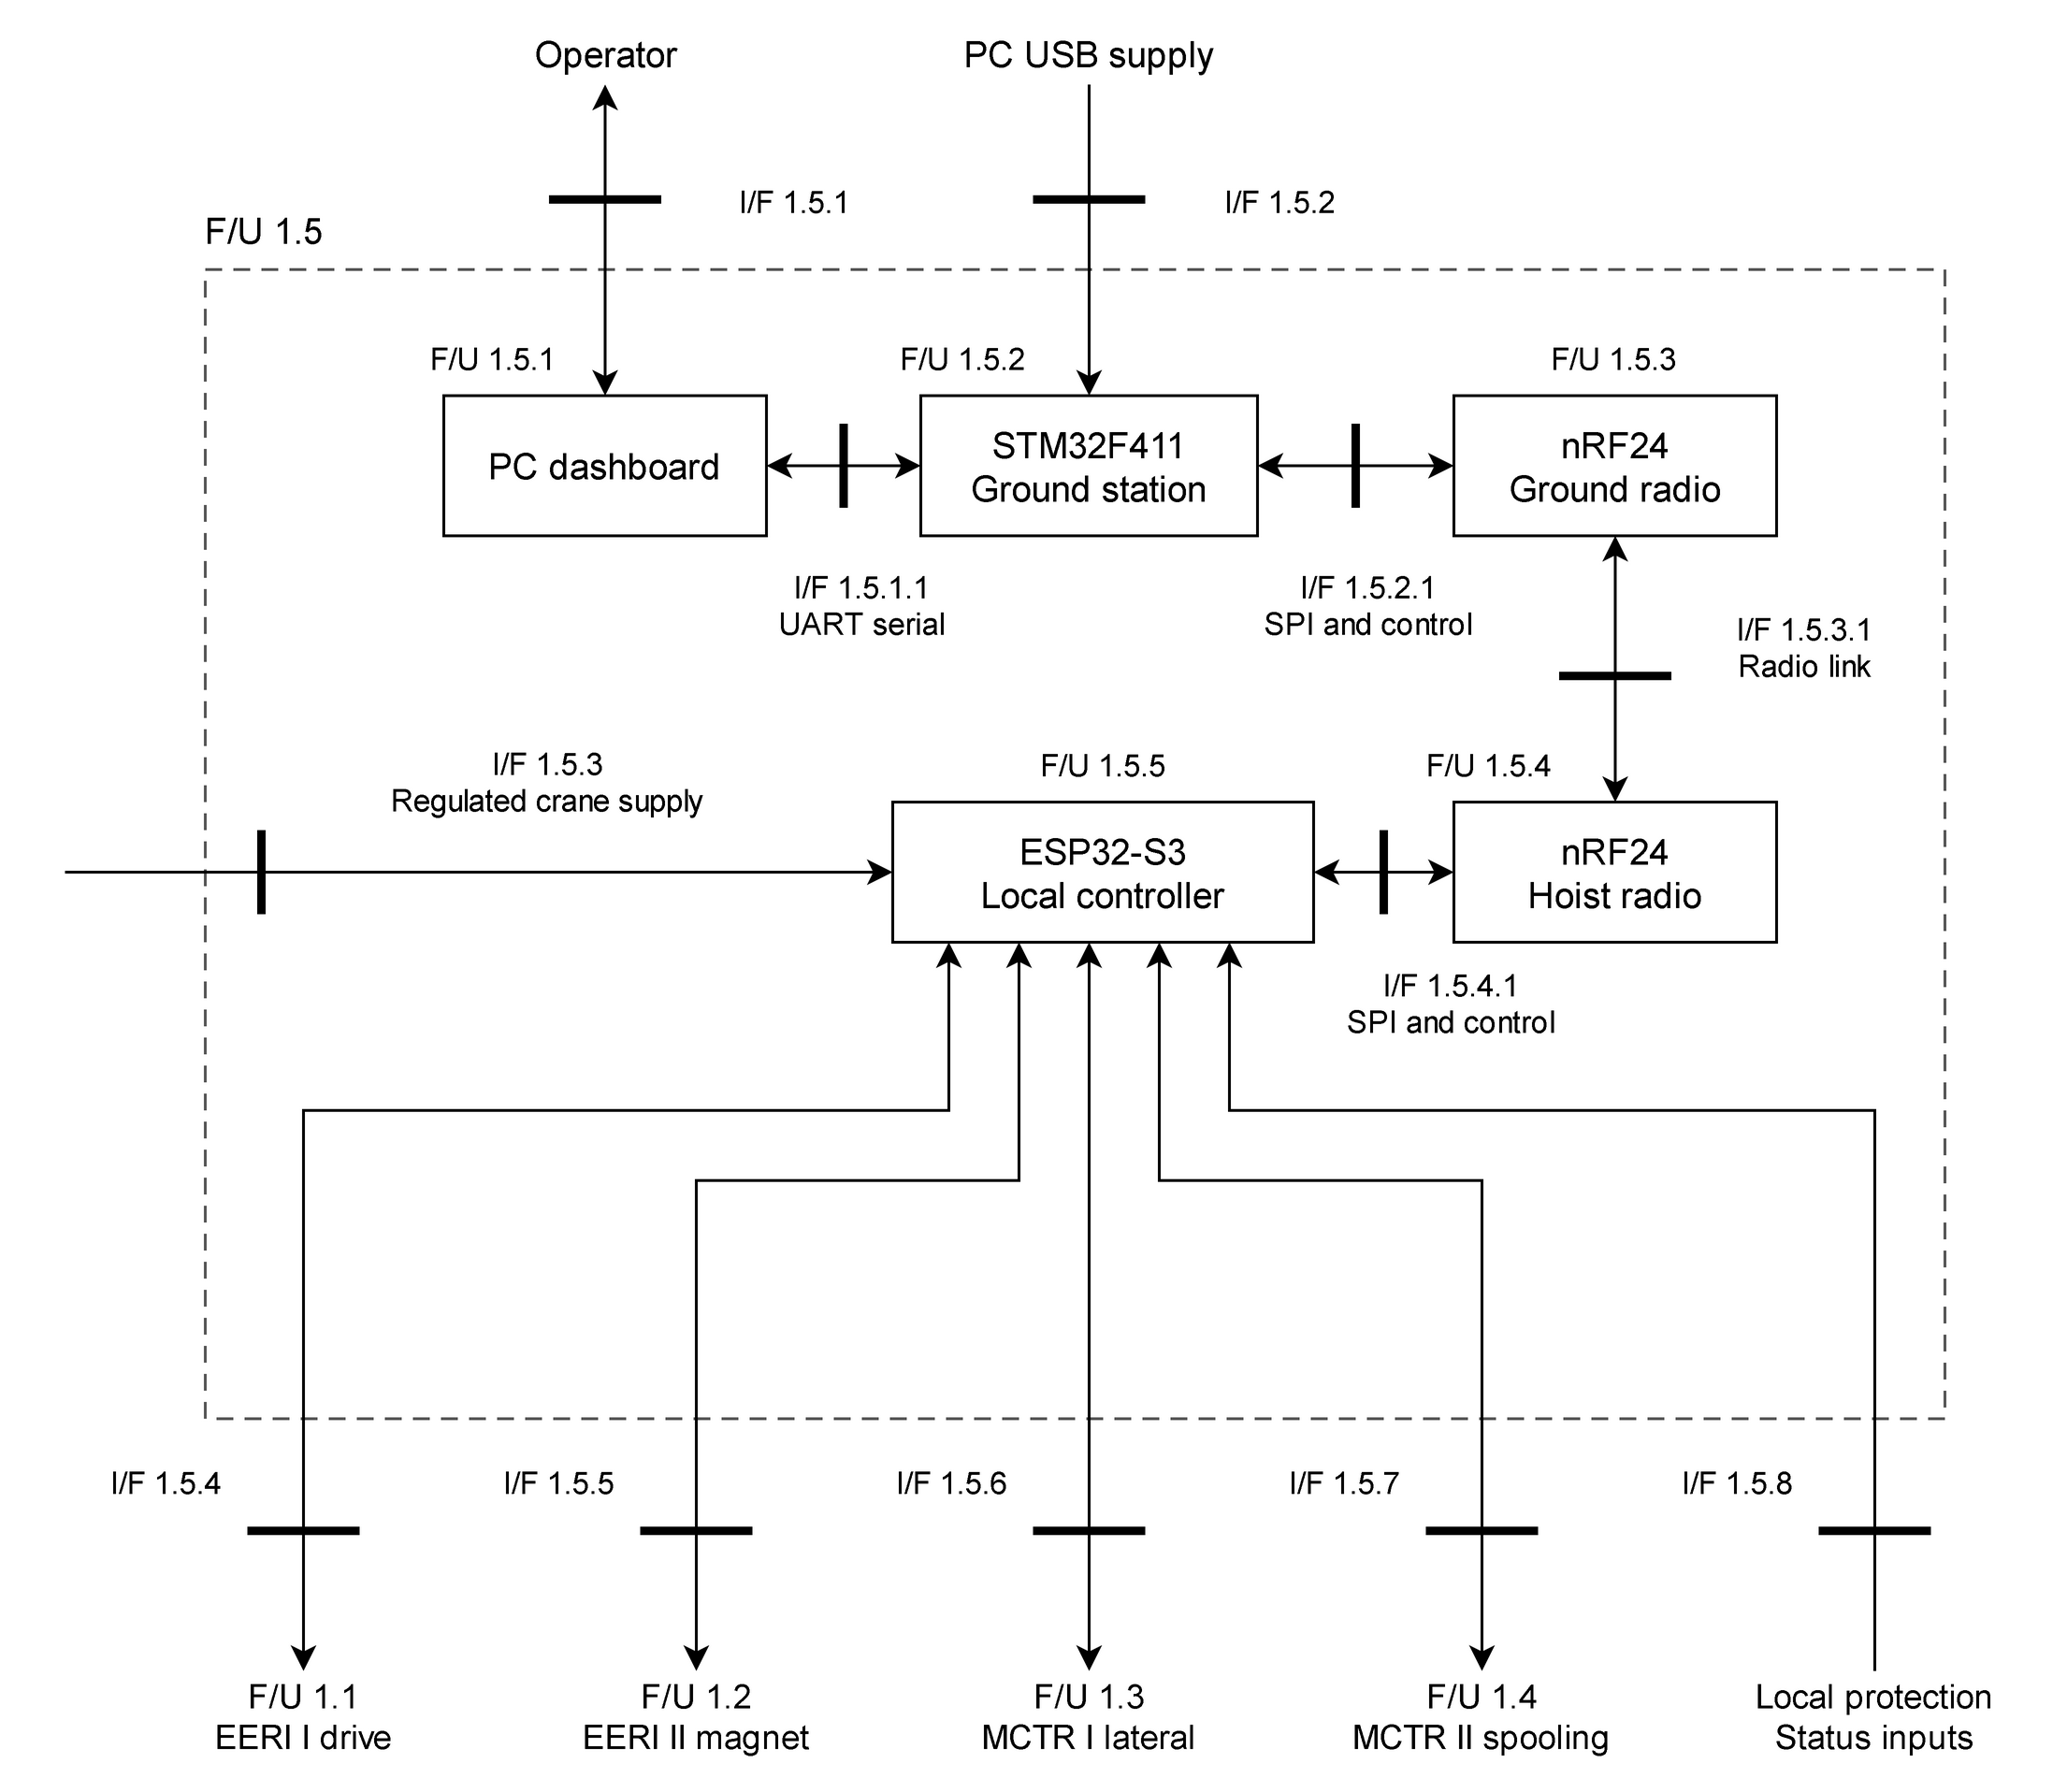
\includegraphics[width=0.85\textwidth]
        {figures/Figure_3_5_System_Architecture.png}
    \caption{Proposed system architecture of REII F/U~1.5.}
    \label{fig:reii-architecture}
\end{figure}

\section{Summary of Interfaces}
\label{sec:summary-of-interfaces}
This section lists each of the interfaces introduced above organised according to their nature, which is either mechanical, electrical, signal, or general. These interfacees are then assigned to each role in chapter \ref{ch:interface-control}.

\subsection{Mechanical Interfaces}
\label{subsec:mechanical-interfaces}
\begin{itemize}
    \item \textbf{EEII I:} I/F 1.8~M connect the 3-phase induction motor to MCTR II (motor shaft to gearbox).
    \item \textbf{MCTR II:} I/F 1.1~M (hoist baseplate to MCTR I mounting plate), I/F 1.3~M (rope to magnetic attachment), I/F 1.8~M (motor shaft to gearbox), and internal I/F \fuMII.1~M (gearbox to drum), \fuMII.3~M (brake to shaft), \fuMII.4~M (rope to load cell).
\end{itemize}

\subsection{Electrical Interfaces}
\label{subsec:electrical-interfaces}
\begin{itemize}
    \item \textbf{EEII I:} I/F 1.0 supplies mains power to the drive electronics subsystem. 
    I/F 1.2 E and I/F 1.6 E supply to the required DC power supplies. I/F 1.7 E provides the 3-phase AC to the
    induction motor.
    \item \textbf{MCTR II:} I/F 1.7~E (motor power from EEII~I) and internal I/F \fuMII.2~E (Brake PSU to brake coil).
\end{itemize}

\subsection{Signal Interfaces}
\label{subsec:signal-interfaces}
\begin{itemize}
    \item \textbf{EEII I:} I/F 1.5 S connects the REII controller to the drive electronics. The controller is
    electrically isolated from the high voltage of the inverter (supplied PWM signbals).
    \item \textbf{MCTR II:} I/F 1.9~S (HX711 to controller), I/F 1.10~S (brake release command) and internal I/F \fuMII.5~S (load cell to HX711).
\end{itemize}

\subsection{General Interfaces}
\label{subsec:general-interfaces}
